\documentclass[oneside, final, 12pt]{extreport}
\usepackage[utf8]{inputenc}
\usepackage[russianb]{babel}
\usepackage{vmargin}
\setpapersize{A4}
\setmarginsrb{2cm}{1.5cm}{1cm}{1.5cm}{0pt}{0mm}{0pt}{13mm}
\usepackage{indentfirst}
\usepackage{graphicx}
\usepackage{amsmath}
\usepackage{amssymb}
%\usepackage[14pt]{extsizes}
\sloppy

\newcommand\Chapter[1]{
	\refstepcounter{chapter}
	\chapter*{
		\begin{huge}
			\textbf{\arabic{chapter}.}
		\end{huge}%
		\bigskip \bigskip
		\raggedright #1
	}
	\addcontentsline{toc}{chapter}{\arabic{chapter}. #1}
}



\begin{document}
	%\fontsize{14}{16pt}\selectfont
	\renewcommand\contentsname{Содержание} %%% renaming the Table of Contents
	%\renewcommand\chaptername{}
	\thispagestyle{empty}
	
	\begin{center}
		\ \vspace{-1cm}
		
		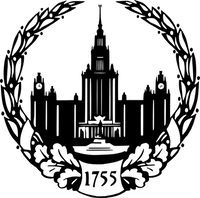
\includegraphics[width=0.2\textwidth]{logo-mgu.png}\\
		{\scshape Московский государственный университет имени М.~В.~Ломоносова}\\
		Факультет вычислительной математики и кибернетики\\
		Кафедра математической кибернетики
		
		\vfill
		
		{\LARGE Курсовая работа по теме}
		
		\vspace{1cm}
		
		{\Huge\bfseries <<Тут должна быть тема>>}
	\end{center}
	
	\vspace{1cm}
	
	\begin{flushright}
		\large
		\textit{Студент 318 группы}\\
		М.\,М. Сакович
		
		\vspace{5mm}
		
		\textit{Научный руководитель}\\
		д.ф-м.н., доцент. С.\,Н. Селезнева
	\end{flushright}
	
	\vfill
	
	\begin{center}
		Москва, 2017
	\end{center}

	\tableofcontents
	\chapter*{Введение}
	\addcontentsline{toc}{chapter}{Введение}
	Деревья принятия решений являются адекватной моделью вычисления, если нужно идентефицировать неизвестный объект из заданного 
	класс, задавая вопросы и получая конечное число ответов. Запросы могут задаваться адаптивно, т.е. вопрос может зависеть от предыдущих 
	ответов. Цель состоит в том, чтобы минимизировать наихудшее число запросов, которое является глубиной дерева решений.
	
	Булевые деревья принятия решений являются наиболее важным подклассом деревьев решений. Известная булева функция $f$ должна быть оценена
	на неизвестном входном наборе $a$. Мы можем запросить биты $a_i$ набора $a$. 	
	По сути, делая запрос, в зависимости от полученного ответа мы переходим в левую или правую часть поддерева. 
	Мерой сложности является количество запросов. Все запросы имееют одинаковую стоимость. Заметим, что минимальная глубина дерева принятия
	решений равна минимальной глубине программ ветвления или диаграмм двоичных решений.\cite{wegener}
	
	Здесь рассматривется еще один класс задач. Дается класс $F$ булевых функций от $n$ переменных и мы хотим выяснить, какие от каких 
	перменных существенно зависит функция $f \in F$.
	
	В статье  \cite{tokio} были получены результаты для классов $OR, PAR$ и $THR$. Класс $OR$ содержит все $OR_S, S \subseteq {1, \ldots, n}$, 
	т.е. дизъюнкция всех $x_i$, где $i \in S$. Фиктивные переменные заменяются константой $0$. Так же рассматривался класс  $OR(k)$, содержащий
	все $OR_s$, где $|S| = k$.\\
	Для классов $OR$ и $OR(k)$ были получены нижние оценки  $n$ и $\lceil \log_2(С_n^k) \rceil$ соответсвенно.
	Класс $OR(k)$ можно распознать за $k\lceil \log_2(\frac{n}{k}) \rceil + 2k - 2$ запроса.\\
	Классы $PAR$ и $PAR(k)$ для функции четности, которая возвращает значение $1$, если число единиц на входе четное, и $0$ иначе. \\
	Для класса $PAR$ нижняя оценка $n$. Для класса $PAR(k)$ был получен алгоритм из $O(k\log_2(\frac{n}{k}))$ запросов. \\
	Классы $THR, THR(k)$ и $THR_t(k)$ порождаются пороговой функцией. Пороговая функция является основой дискретных нейронных сетей.
	Пороговое значение $t$ определяет, сожержит ли вход по крайней мере $t$ единиц. Для классов $THR$ и $THR(k)$ пороговое значение неизвестно.
	Нижние оценки для классов $THR, THR(k)$ и $THR_t(k)$ равны $n-1 + \lceil \log_2(n+1) \rceil, \lceil \log_2(kC_n^k + 2) \rceil$ и $\lceil \log_2(C_n^k) \rceil$ 
	соответсвенно. Так же были получены алгоритмы: за $n-1 + \lceil \log_2(n+1) \rceil$ запросов для $THR$, за 
	$2(k-1)\log_2(\frac{n-1}{k-1}) + 6k - 6 + \lceil \log_2(n+2) \rceil$ запросов для $THR(k)$ и за $(k-1)\log_2(\frac{n-1}{k-1}) + 3k - 3 + \lceil \log_2(n+2) \rceil$ 
	запросов для $PAR_t(k)$.
	
	В данной работе рассмотрим еще несколько классов: $A_0, A_1, A_2$.
	
	\Chapter{Основные определения}
	\noindent\emph{Определение.} Набор $(\alpha_1, \alpha_2, \ldots, \alpha_n)$, где $\alpha_i \in \{0,1\}, 1\leq i \leq n$, называется булевым или двоичным 
	набором (вектором). Элементы набора называют координатами. Число $n$ называется длинной набора. Далее двоичный набор длины $n$ будем 
	обозначать $\tilde{\alpha}$.\cite{gavrilov:sapogenko}\\
	\noindent\emph{Определение.} Множество всех двоичных наборов длины $n$ образует $n$-мерный булев(или двоичный) куб, который называют 
	также единичным $n$-мерным кубом и обычно обозначают $B^n$.\cite{gavrilov:sapogenko}\\
	\noindent\emph{Определение.} Весом (или нормой) набора $\tilde{\alpha}$ (обозначение $ \| \tilde{\alpha} \| $) называют число его координат, 
	равных $1$, т.е.  $$ \| \tilde{\alpha} \| = \sum_{i=1}^{n} \alpha_i.\cite{gavrilov:sapogenko} $$\\
	\noindent\emph{Определение.} Наборы $\tilde{\alpha} \in B^n$ называют вершинами куба $B^n$. Множество всех вершин куба $B^n$, имеющих вес 
	$k$, называется $k$-м слоем куба  $B^n$ (обозначение $B_k^n$).\cite{gavrilov:sapogenko}\\
	\noindent\emph{Определение.} Набор, вес которого  равен $0$, будем называть нулевым набором. Набор, вес которого равен $n$, будем 
	называть единичным набором.\\
	\noindent\emph{Определение.} Наборы будем называть соседними, если они различаются только в одной координате.\\
	\noindent\emph{Определение.} Функция $f(x_1, \ldots, x_n)$, определенная на множестве $B^n = \{0,1\}^n$ и принимающая знаечения из множества 
	$\{0, 1\}$, называется функцией алгебры логики (булевой функцией). Множество всех булевых функций обозначим $P_2$. \cite{gavrilov:sapogenko}\\
	\noindent\emph{Лемма.} Мощность множества $P_2$ равна   $2^{2^n}$.\\
	\noindent\emph{Определение.} Переменная $x_i \: (1 \! \leq \! i \!  \leq \! n)$ функции $f(x_1, \ldots, x_{i-1}, x_i, x_{i+1}, \ldots, x_n)$ называется существенной, 
	если можно указать такие наборы $\tilde{\alpha}$ и $\tilde{\beta}$, соседние по $i$-ой компоненте, 
	(т.е $\tilde{\alpha} = (\alpha_1, \ldots, \alpha_{i-1}, 0, \alpha_{i+1}, \ldots, \alpha_n)$ и 
	$\tilde{\beta} = (\alpha_1, \ldots, \alpha_{i-1}, 1, \alpha_{i+1}, \ldots, \alpha_n)$), 
	что $f(\tilde{\alpha}) \not= f(\tilde{\beta})$.
	В противном случае переменная назывется фиктивной. Если у функции все переменные фиктивные, то она считается константой. \cite{gavrilov:sapogenko}\\
	\noindent\emph{Определение.} Запросом $\alpha$ для функции $f(x)$ будем называть проверку значения $f(\alpha)$. \\
	\noindent\emph{Теорема.} Нижняя оценка для класса $F$, мощности $|F|$, равна $\lceil \log_2(|F|) \rceil$. \\
	\noindent\emph{Теорема.} Для всех $n \ge 1$ верно 
	\[ 
		\sum_{k=0}^{n}C_n^k = 2^n. \cite{selezneva}
	\]
	
	\noindent\emph{Теорема.} Средняя сложность алгоритма бинарного поиска $L^{cp}(n) \leq \log_2(n)$. \cite{alekseev}
	
	\Chapter{Основная часть}
	\section{Постановка задачи}
	Введем функцию 
	\[ \tau_i(x) = \begin{cases}
		1, & \|\tilde{\alpha}\| mod 3 = i \\
		0, & \|\tilde{\alpha}\| mod 3 \not = i
	\end{cases}\]
	
	Будем рассматримвать три функции: $\tau_0(x), \tau_1(x), \tau_2(x)$, каждая из которых порождает классы $A_0, A_1, A_2$ соответсвенно.
	Попытаемся  узнать, от каких перменных существенно зависит функция $f \in A_i, i = 0, 1, 2$.
	
	\noindent Задача состоит в том, чтобы узнать, достигается ли нижняя оценка для классов $A_0, A_1, A_2$, и построить алгоритм, для которого она 
	достигается.
	
	\section{Решение} 
	\noindent Чтобы дать нижнюю оценку, посчитаем мощность классов $A_0, A_1, A_2$.\\
	\noindent\emph{Лемма}. Мощность классов $A_0$ и $A_1$ равна $2^n$.\\
	\noindent\emph{Доказательство}. Рассмотрим класс $A_0$. Он порождается функцией $\tau_0(x)$, зависящей от $n$ переменных. Из этих $n$ переменных 
	можем выбрать $0$ существенных переменных, т.е. $C_n^0$, $1$ существенную перменную, т.е. $C_n^1$ и.т.д..
	Таким образом, 
	\[
		|A_0| = C_n^0 + C_n^1 + \cdots + C_n^n = \sum_{k=0}^{n}C_n^k = 2^n.
	 \]	
	
	\noindent Аналогично, $|A_1| = 2^n $. $\blacksquare$ \par
	\bigskip
	\noindent\emph{Лемма}. Мощность класса $A_2$ равна $2^n - n$.\\
	\noindent\emph{Доказательство}. Класс $A_2$ порождается функцией $\tau_2(x)$, которая завивит от $n$ переменных. В отличии от классов $A_0$ и $A_1$,
	если функция из класса $A_2$  существенно зависит от одной переменной, то она никогда не примет значение 1, значит мы не сможем распознать её. Таким образом 
	\[
		|A_2| = C_n^0 + C_n^2 + \cdots + C_n^n = \sum_{k=0}^{n}C_n^k - C_n^1 = 2^n - n. \blacksquare
	\]
	
	\noindent Зная мощности классов, можно дать нижнюю оценку 
	\begin{displaymath}
		\begin{aligned}
			1. \lceil \log_2{|A_0|} \rceil & = \log_2{2^n} = n  \\		
			2. \lceil \log_2{|A_1|} \rceil & = \log_2[2^n] = n  \\
			3. \lceil \log_2{|A_2|} \rceil & = \lceil \log_2{2^n - n} \rceil.  \\
		\end{aligned}
	\end{displaymath}
	
	\noindent Посмотрим, достигаюся ли нижние оценки для классов $A_0, A_1, A_2$. \par
	\bigskip
	\noindent Построим алгоритм из $n$ запросов  для функции из класса  $A_0$.
	
	\noindent\emph{Решение}. \\
	\emph{Шаг} 1. Рассмотрим функцию $f$  из класса $A_0$ на нулевом наборе
	 \[
	 	\tau_0(0, 0, \ldots, 0) =  \{0 \, mod \, 3 = 0\} = 1.
	 \]
	 Не задавая вопроса, мы знаем, что любая функция из класса $A_0$ на нулевом наборе имеет значение $1$.\\
	 \emph{Шаг} 2. Рассмотрим набор $\alpha_1 = (1, 0,  \ldots, 0)$. Если $f(\alpha_1) = 1$, то переменная $x_1$ не влияет на значение функции, т.е. $x_1$ - 
	 фиктивная переменная, в противном случае $x_1$ - существенная \\
	 \emph{Шаг} 3. Теперь рассмотрим набор $\alpha_i = (0, \ldots, 0,  1,  0, \ldots, 0)$, в котором на $i$-м месте стоит $1$, а на всех остальных местах $0$.
	  Применяя аналогичные рассуждения узнаем, является ли переменная $x_i$ существенной. Применим шаг 3. для всех $i = 2, 3, \ldots, n$. \\ 
	 \noindent Т.о. делаем $n$  запросов $\alpha_1, \alpha_2, \ldots, \alpha_n$ и для каждой из перменных $x_1, x_2, \ldots, x_n$ узнаем, является она существенной 
	 или фиктивной.\par
	\bigskip
	\noindent Построим алгоритм из $n$ запросов  для функции из класса  $A_1$.
	
	\noindent\emph{Решение}. \\
	\emph{Шаг} 1. Рассмотрим функцию $f$  из класса $A_1$ на нулевом наборе
	\[
		\tau_1(0, 0, \ldots, 0) =  \{0 \, mod \, 3 = 0\} = 0.
	\]
	Из этого следует, что не задавая вопроса, мы знаем, что любая функция из класса $A_1$ на нулевом наборе имеет значение $0$.
	Заметим, что если функция $f$ существенно зависит от всех своих переменных, то на любом наборе из первого слоя, функция $f$ принимает значение $1$.\\
	\emph{Шаг} 2. Рассмотрим набор $\alpha_1 = (1, 0,  \ldots, 0)$. Если $f(\alpha_1) = 0$, то переменная $x_1$ не влияет на значение функции, т.е. $x_1$ - 
	фиктивная переменная, в противном случае $x_1$ - сущесвтенная \\
	\emph{Шаг} 3. Теперь рассмотрим набор $\alpha_i = (0, \ldots, 0,  1,  0, \ldots, 0)$, в котором на $i$ -м месте стоит $1$, а на всех остальных местах $0$.
	 Применяя аналогичные рассуждения узнаем, является ли переменная $x_i$ существенной. Применим шаг 3. для всех $i = 2, 3, \ldots, n$. \\
	\noindent Т.о. делаем $n$  запросов $\alpha_1, \alpha_2, \ldots, \alpha_n$ и для каждой из перменных $x_1, x_2, \ldots, x_n$ узнаем, является она существенной 
	или фиктивной.\par
	\bigskip
	\noindent Построим алгоритм распознавания функции из класса $A_2$  \\
	\emph{Шаг} 1. Рассмотрим функцию $f$ из класса $A_2$  на наборе $\tilde{\alpha} = (1, 1, 0, \ldots, 0)$. Если $f(\tilde{\alpha}) = 1$, то переходим к шагу 3. В противном
	случае переходим к шагу 2. \\
	\emph{Шаг} 2. Заменим в  наборе $\tilde{\alpha}$ первый встречающийся $0$ на  $1$. Если $f(\tilde{\alpha}) = 1$, то переходим к шагу 3. Если набор
	 $\tilde{\alpha}$ - единичный и $f(\tilde{\alpha}) = 0$, то все переменные функции $f$ - фиктивные, иначе повторяем шаг 2.\\
	\emph{Шаг} 3. Не нарушая общности рассуждений, пусть последняя единица в наборе $\tilde{\alpha}$ стоит на $k$-м месте ($k \leq n$).
	 Обозначим такой набор как $\tilde{\alpha_k}$. Тогда переменная  $x_k$ - существенная.
	 Среди переменных $x_1, x_2, \ldots, x_{k-1}$ ровно одна существенная, т.к. $\tau_2(\tilde{\alpha})$ может принять первый раз значение $1$ только в 
	 том случае, если на месте двух первых встретившихся существенных переменных в наборе $\tilde{\alpha}$ стоят единицы, 
	 а так как добавление единицы на $k$-е место обращает функцию $\tau_2(\tilde{\alpha})$ в $1$, то $x_k$ -  вторая существенная переменная, 
	 а первая нахоится среди первых $k-1$ переменных. \\
	\emph{Шаг} 4. Найдем первую существенную переменную. Для этого построим набор 
	$${\alpha_{\lceil \frac{k-1}{2}\rceil_{k-1}}} = (1, 1, \ldots, 1, 0, \ldots, 0, 1, 0, \ldots, 0),$$
	 который получается из набора $\tilde{\alpha}$ заменой $1$, стоящих на местах $\lceil \frac{k-1}{2} \rceil, \lceil \frac{k-1}{2} \rceil + 1, \ldots, k-1$ на $0$. \\
	 Если $f({\alpha_{\lceil\frac{k-1}{2}\rceil_{k-1}}}) = 0$, то существенная переменная находится среди $x_{\lceil\frac{k-1}{2}\rceil}, \ldots, x_{k-1}$, в противном
	 случае существенная переменная среди $x_1, \ldots, x_{\lfloor \frac{k-1}{2} \rfloor}$. Т.о мы сузили область поиска вдвое. Аналогичным образом 
	 будем заменять половину оставшихся $1$ на $0$, в зависимости  того, в какую половину попадает существенная переменная, до тех пор, пока не останется 
	 одна $1$, соответсвующая переменной $x_i$. \\
	 Переменная $x_i$ - является существенной. Пусть $\alpha_{ik} = (0, \ldots,0, 1, 0, \ldots, 0, 1, 0, \ldots, 0)$, где на $i$-м и  $k$-м местах стоят $1$, а на всех 
	 остальных $0$. Т.к. $x_i$ и $x_k$ - существенные, то  $f(\alpha_{ik}) = 1$. \\
	 \emph{Шаг} 5. Осталось найти все существенные переменные среди $n-k$ оставшихся. Для этого составим $n-k$ запросов: 
	 \begin{displaymath}
	 \begin{aligned}
	 	\alpha_{ik_1} & = (0, \ldots,0, 1, 0, \ldots, 0, 1, 1, 0, \ldots, 0) \\
	 	\alpha_{ik_2} & = (0, \ldots,0, 1, 0, \ldots, 0, 1, 0, 1, \ldots, 0) \\
	 	                    & \cdots \\
	 	\alpha_{ik_n} & = (0, \ldots,0, 1, 0, \ldots, 0, 1, 0, 0, \ldots, 1)
	 \end{aligned}
	 \end{displaymath}
	
	Если $f(\alpha_{ik_j}) = 1$ (где $j = k+1, \ldots, n$), то переменная $x_j$ - фиктивная. В противном случае $x_j$ - существенная.\\
	Посчитаем, сколько запросов нам понадобилось. \\
	На первом шаге 1 запрос. На втором шаге нам понадобилось $k-2$ запроса, где $k \leq n$. На 5-м шаге  $n-k$. Четвертый шаг по сути является
	алгоритмом бинарного поиска, сложность которого $ \leq \log_2(n)$. Таким образом, в худшем случае сложность приведенного алгоритма равна 
	$1 + k - 2 + n - k + \log_2(n) = n - 1 + log_2(n)$. Ассимптотическая сложность: $n + o(n)$.
	
	\section{Результаты}
	
	Для классов $A_0$ и $A_1$ получена оптимальная оценка в $n$ шагов, которая достигается на представленом алгоритме. Для класса $A_2$ получена оценка
	$\lceil \log_2{2^n - n} \rceil$ и представлен алгоритм с ассимптотической сложностью $n + o(n)$.
	
	\begin{thebibliography} {0}
		\addcontentsline{toc}{chapter}{Литература}
		
		\bibitem{wegener} Ingo Wegener \emph{The complexity of boolean functions.} Wiley-Teubner, 1987.
		
		\bibitem{tokio} Ryuhei Uehara, Kensei Tsuchida, Ingo Wegener \emph{Optimal attribute-efficient learning of disjunction, parity, and threshold functions}. 1996.
		
		\bibitem{gavrilov:sapogenko} Гаврилов Г.П., Сапоженко А.А. \emph{Сборник задач по дискретной математике.} М.:ФИЗМАТЛИТ, 2004.
		
		\bibitem{selezneva} Слезнева С.Н. \emph{Лекции по "Избранным вопросам дискретной математики" 3-й курс, 318 группа.} 2016.
		
		\bibitem{alekseev} Алексеев В.Б. \emph{Введение в теорию сложности алгоритмов.} М.: Изд. отдел ф-та ВМиК МГУ, 2002.
		
	\end{thebibliography}
\end{document}
